\documentclass[9pt, aspectratio=169]{beamer}
\usepackage{FiraSans}
\usetheme[subsectionpage=progressbar]{metropolis}
\usepackage[utf8]{inputenc}
\usepackage{amsmath}
\usepackage{amsfonts}
\usepackage{amssymb}
\usepackage{multicol}
\usepackage{tikz}
\usetikzlibrary{shapes.geometric, positioning}
\usepackage{caption}
\usepackage{xcolor}
\usepackage[T1]{fontenc} 
\usepackage[skins]{tcolorbox}
\author{Nicola Roman\`o - nicola.romano@ed.ac.uk}
\title{Lecture 15 - Using Keras to build a CNN}
\setlength{\fboxsep}{0pt}
\setbeamertemplate {footline}{\begin{scriptsize}\hfill\insertframenumber ~of \inserttotalframenumber\kern1em\vskip5pt\end{scriptsize}}

% Remove "Figure" in front of captions
% See https://tex.stackexchange.com/questions/82456/how-to-remove-figure-caption-prefix-figure-in-beamer
\captionsetup{labelformat=empty,labelsep=none}

\titlegraphic{\centering 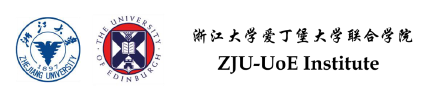
\includegraphics[scale=.5]{instituteLogo.png}}
\date{}

\begin{document}

\newtcolorbox{codebox}{enhanced,
    top=2pt,
    left=2pt,
    right=2pt,
    bottom=2pt,
    boxrule=0pt,
    leftrule=5pt,
    sharp corners,
    colback=gray!20,
    colframe=blue!60!black}

\begin{frame}
    \titlepage
\end{frame}

\begin{frame}
    {Learning objectives}
    \begin{columns}
        \begin{column}{0.8\textwidth}
            \begin{itemize}
                \item Describe tools commonly used to build a CNN.
                \item Use Keras for building and training a "\textit{LeNet-5 style}" CNN.
                \item Use Keras for transfer learning.
            \end{itemize}
        \end{column}
        \begin{column}{0.2\textwidth}
            
\includegraphics[angle=-30, origin=tr, width=1.5\textwidth]{lightbulb.png}
        \end{column}
    \end{columns}
\end{frame}

\section{The tools}

\begin{frame}
    {Python tools for deep learning}

    \begin{columns}
        \begin{column}{.3\textwidth}
            \centering
            
\includegraphics[width=\textwidth]{tf_keras_pythorch_logo.png}
        \end{column}

        \begin{column}{.7\textwidth}
            \textbf{TensorFlow}
            \begin{itemize}
                \item \textit{"An end-to-end open source platform for machine learning"}
                \item Developed by Google
            \end{itemize}

            \textbf{PyTorch}
            \begin{itemize}
                \item \textit{"An open source machine learning framework"}
                \item Developed by Facebook
            \end{itemize}

            \textbf{Keras}
            \begin{itemize}
                \item \textit{"A deep learning framework"}
                \item Developed by Fran\c{c}ois Chollet (package \texttt{keras}).
                \item The \texttt{keras} package also supports other "backends" (like JAX or Pythorch).
            \end{itemize}
        \end{column}
    \end{columns}
    \raggedright

    \vspace{1em}
    \centering
    For this course we will use \textbf{Keras version 3}, but feel free to explore PyTorch as well!
\end{frame}

\begin{frame}
    {A very brief overview of Keras}
    \centering
    \begin{tikzpicture}[scale=.8]
        % Keras logo at the center
        \node[inner sep=0pt] (keras) at (0,0)
        {
\includegraphics[height=1cm]{keras_logo.png}};

        % Define radius and number of nodes
        \def\radius{4}
        \def\nodes{7}

        % Place the nodes in a circle around the Keras logo
        \foreach \i [count=\n] in {Models, Layers, Optimizers, Losses, Metrics, Callbacks, \dots} {
                \node[draw, fill=white, align=center, text width=1.5cm, minimum height=1cm] (node\n) at ({360/\nodes*\n}:\radius) {\i};
            }

        % Add the "Other" node
        \node[draw, fill=white, align=center, text width=1.5cm, minimum height=1cm] (other) at ({360/\nodes*7}:\radius) {\dots};

        % Arrows from keras to each node
        \foreach \n in {1,...,7} {
                \draw[->] (keras) -- (node\n);
            }

        % Add explanations next to each node
        \node[text width=2.2cm, minimum height=1cm, anchor=north west, align=center] (model_explanation) at ({360/7*1}:\radius+2) {\texttt{Model} and \texttt{Sequential} classes - define a model};
        \node[text width=3.2cm, minimum height=1cm, anchor=east, align=center] (layer_explanation) at ({360/7*2.2}:\radius+1) {Define various types of ANN layers};
        \node[text width=2.2cm, minimum height=1cm, anchor=north east, align=center] (optimizer_explanation) at ({360/7*3}:\radius+1) {Optimizers for training};
        \node[text width=2.2cm, minimum height=1cm, anchor=east, align=center] (loss_explanation) at ({360/7*4}:\radius+1.5) {Loss functions};
        \node[text width=4.4cm, minimum height=1cm, anchor=east, align=center] (metrics_explanation) at ({360/7*4.9}:\radius+0.5) {Metrics for\\evaluating the model};
        \node[text width=4cm, minimum height=1cm, anchor=west, align=center] (callbacks_explanation) at ({360/7*6}:\radius+1) {Functions to perform actions during training};
        \node[text width=2.2cm, minimum height=1cm, anchor=west, align=center] (other_explanation) at ({360/7*7}:\radius+1.5) {Other modules};
    \end{tikzpicture}

\end{frame}

\begin{frame}
    {Layers}
    Keras makes it easy to define layers.

    Several classes are available, such as \texttt{Conv2D}, \texttt{MaxPooling2D}, \texttt{Dense}, etc.

    \pause
    \vspace{1em}

    \begin{columns}[t]
        \begin{column}{.5\textwidth}
            \textbf{Convolutional layer}
            \begin{itemize}
                \item 32 filters
                \item Size of 3x3, stride of 1, valid padding
                \item ReLU activation
            \end{itemize}

            \vspace{1em}
            \begin{codebox}
                \texttt{layer = keras.layers.Conv2D(\\
                    $~~~~$filters=32,\\
                    $~~~~$kernel\_size=3, strides=(1,1), $~~~~$padding='valid',\\ $~~~~$activation='relu')
                }
            \end{codebox}
        \end{column}

        \pause

        \begin{column}{.5\textwidth}
            \textbf{Dense layer}
            \begin{itemize}
                \item 128 units
                \item Sigmoid activation
            \end{itemize}

            \vspace{2.5em}
            \begin{codebox}
                \texttt{layer = keras.layers.Dense(\\
                    $~~~~$units=128, activation='sigmoid')}
            \end{codebox}
        \end{column}
    \end{columns}
\end{frame}

\begin{frame}
    {Keras models}
    Two ways to build a model.
    \vspace{2em}

    \begin{columns}[t]
        \begin{column}{.45\textwidth}
            \textbf{Sequential API}
            \begin{itemize}
                \item A sequential model is a linear stack of layers.
                \item You can add layers one at a time using the \texttt{add} method.
            \end{itemize}

            \vspace{1em}
            \begin{codebox}
                \texttt{model = keras.models.Sequential()\\
                    model.add(layer)\\
                    model.add(layer2)}
            \end{codebox}
        \end{column}

        \begin{column}{.55\textwidth}
            \textbf{Functional API}
            \begin{itemize}
                \item For non-linear, more complex models
                \item Allows multiple inputs and outputs
            \end{itemize}

            \vspace{1em}
            \begin{codebox}
                \texttt{input\_img = keras.Input(shape=(28, 28, 3))\\
                    FC = keras.layers.Dense(units=50)(input\_img)\\
                    out = keras.layers.Dense(units=5)(FC)\\
                    model = keras.Model(inputs = input\_img,\\ $~~~~$outputs = out)
                }
            \end{codebox}
        \end{column}
    \end{columns}
\end{frame}

\begin{frame}
    {Compiling the model}
    Once the model has been created it needs to be \textit{compiled}. This allows us to choose the optimizer, the loss function and the metrics to monitor during training.

    For example, for a classification problem, we might decide to use stochastic gradient descent$^*$ as the optimizer, cross entropy as the loss function and accuracy as the metric.

    \footnotesize
    $^*$Note: Adam (ADAptive Movement estimation algorithm, Diederik et al, 2014), is an implementation of the stochastic gradient descent algorithm often used in deep learning.

    \vspace{2em}
    \normalsize
    \begin{codebox}
        \texttt{model.compile(optimizer='adam',\\
        $~~~~$loss='categorical\_crossentropy',\\
        $~~~~$metrics=['accuracy'])}
    \end{codebox}

    \normalsize
    Great! We're all set for training!
\end{frame}

\begin{frame}
    {Training}
    At training time, we need to feed the model with data.
    We will have defined some \textbf{training} and \textbf{validation} set.

    Now we need to set:
    \begin{itemize}[<+->]
        \item \textbf{Epochs}. How many times to go through all the training data.
        \item \textbf{Batch size}. Training with all the data at once (\textit{batch training}) is computationally expensive. Using \textbf{mini-batches} is faster, but might need more epochs.
        \item Example: 1000 training samples, \texttt{batch\_size = 100}. It will take 10 \textbf{iterations} to complete one epoch.
        \item The special case of \texttt{batch\_size=1} is \textbf{stochastic gradient descent} (SGD).
        \item A forward and a backward pass are  run for each \underline{iteration}.
    \end{itemize}

    \only<2>{
        \centering
        \vspace{-4em}
        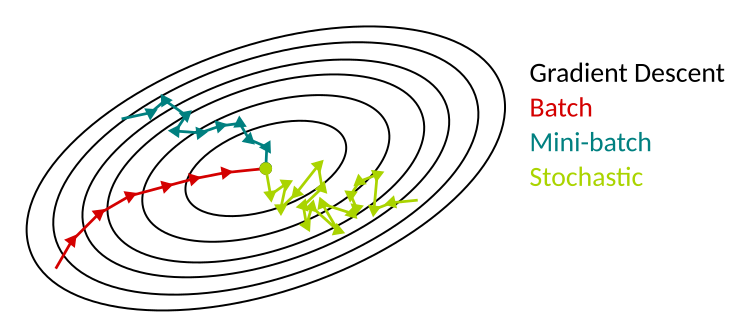
\includegraphics[width=0.7\textwidth]{gradient_descent.png}
    }
\end{frame}

\begin{frame}
    {Training - code}
    \begin{codebox}
        \texttt{history = model.fit(x\_train, y\_train,\\
            $~~~~$batch\_size=32,\\
            $~~~~$epochs=10,\\
            $~~~~$validation\_data=(x\_val, y\_val))}
    \end{codebox}

    \normalsize
    \textbf{Note:}
    \begin{itemize}
        \item The \texttt{fit} method takes as input the training data, the labels and the number of epochs to train for.
        \item The \texttt{fit} method returns a history object, which contains the loss and accuracy values for each epoch.
    \end{itemize}
\end{frame}

\begin{frame}
    {And now... predict!}
    Prediction is as simple as calling the \texttt{predict} method on the model.

    \begin{codebox}
        \texttt{predictions = model.predict(x\_test)}
    \end{codebox}
\end{frame}

\section{Example 1 - A ``\textit{LeNet-5 style}'' CNN}

\begin{frame}
    {Example 1 - A simple CNN}
    Remember the LeNet-5 CNN architecture

    \centering
    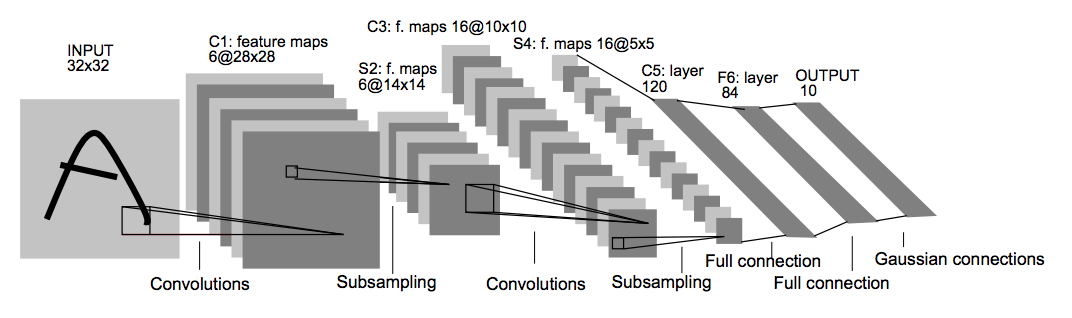
\includegraphics[width=\textwidth]{lenet5.png}

    We are going to build a similar version, to train on the MNIST dataset. We are "remodernising" it by using ReLU activations, max pooling and a softmax output layer.
\end{frame}

\section {Example 2 - Transfer learning}

\begin{frame}
    {Transfer learning}
    \centering
    \begin{tikzpicture}[scale=0.9]
        % Generic images
        \node[inner sep=0pt] (generic) at (0,2)
        {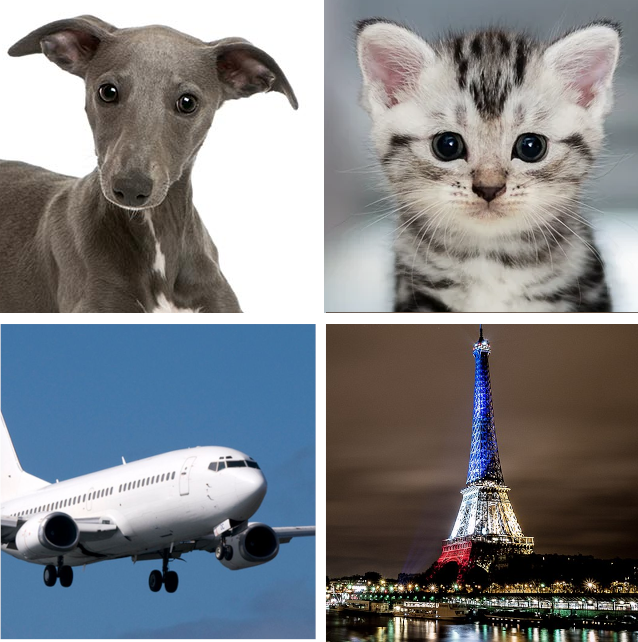
\includegraphics[height=2.5cm]{genericimages.png}};
        \node (label) at (0, 0) {Generic images};

        % Top CNN
        % Conv layers
        \foreach \x [count=\N] in {2.5,3,...,5}
            {
                \node (layer\N) [draw, rectangle, fill=orange!50!yellow, minimum width=1, minimum height=3cm-0.4*\N cm] at (\x,1.5) {};
            }
        % FC layers
        \foreach \x [count=\N from 7] in {6,6.5,7}
            {
                \node (layer\N) [draw, rectangle, fill=blue!50!yellow, minimum width=1, minimum height=2.5cm-.1*\N cm] at (\x,1.5) {};
            }
        \node [text width=4em] (layer10) at (9.5, 1.5) {Dog, Cat, Plane, \dots};
        % Arrows
        \foreach \N [count=\Nn from 2] in {1,2,...,9}
            {
                \draw [->] (layer\N) -- (layer\Nn.west);
            }
        \node [right of=label, node distance=6cm] {\textit{"Template"} CNN - e.g. VGG-16};

        % Domain specific images
        \node[inner sep=0pt] (generic) at (0,-2)
        {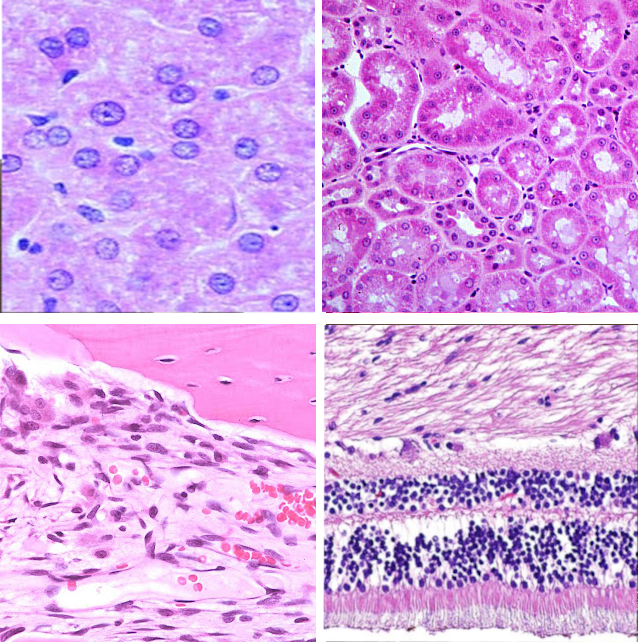
\includegraphics[height=2.5cm]{bioimages.png}};
        \node at (0, -4) {Task-specific images};

        % Bottom CNN
        % Conv layers
        \foreach \x [count=\N] in {2.5,3,...,4.5}
            {
                \node (layer_bottom_\N) [draw, rectangle, fill=orange!50!yellow, minimum width=1, minimum height=3cm-0.4*\N cm] at (\x,-2) {};
            }
        \node (layer_bottom_6) [draw, rectangle, fill=green!40!yellow, minimum width=1, minimum height=0.6cm] at (5,-2) {};

        % FC layers
        \foreach \x [count=\N from 7] in {6,6.5,7}
            {
                \node (layer_bottom_\N) [draw, rectangle, fill=green!60!yellow, minimum width=1, minimum height=2.5cm-.1*\N cm] at (\x,-2) {};
            }

        \node [text width=4em] (layer_bottom_10) at (9.5, -2) {Liver, Kidney, Bone, Retina, \dots};
        \node [color=orange!80!black] at (4, 4) {\textbf{Conv layers}};
        \node [color=blue!50!yellow] at (6.5, 4) {\textbf{FC layers}};
        \draw [color=orange, line width=1pt] (2.2,-3.7) -- (4.8,-3.7) node [below, midway] {Keep};
        \draw [color=green!50!black, line width=1pt] (5,-3.7) -- (8,-3.7) node [below, midway] {Retrain};
        % Arrows
        \foreach \N [count=\Nn from 2] in {1,2,...,9}
            {
                \draw [->] (layer_bottom_\N) -- (layer_bottom_\Nn.west);
            }
    \end{tikzpicture}
\end{frame}

\begin{frame}
    {Transfer learning - VGG16 on CIFAR-10}
    We are going to use the pretrained VGG16 weights to classify the CIFAR-10 dataset.

    The CIFAR-10 dataset consists of 60000 32x32 color images in 10 classes, with 6000 images per class.
\end{frame}

\end{document}

